\chapter{Diseño e implementación}
\pagenumbering{arabic}

\section{Redes neuronales recurrentes de tiempo continuo (CTRNN)}
En contraste con las redes neuronales feed-forward, las cuales soportan únicamente comportamientos
reactivos, en las Redes Neuronales Recurrentes de Tiempo Continuo (CTRNN) (Beer,
1995a) pueden existir ciclos en su estructura y la activación de sus neuronas es asíncrona y multiescalada
en el tiempo. Este tipo de redes neuronales también facilita describir el agente como un
sistema dinámico acoplado al entorno en el que está ubicado, ya que está demostrado que son el
modelo más simple de red neuronal dinámica continua no lineal (Funahashi y Nakamura, 1993).
Además, la interpretación neurobiológica de las CTRNN ha sido demostrada y puede consultarse
en (Beer, 1995a).

\subsubsection{Descripción matemática de una CTRNN}
Las CTRNN están formadas por neuronas cuyo comportamiento se describe en las ecuaciones 3.1 y 3.2
\begin{equation} \label{eq:funcionCTRNN}
	\dot{y_{i}}= \frac{1}{\tau_{i}} * \left ( -y_{i}+\sum_{j=1}^{N}w_{ji}*\sigma \left ( y_{j} + \theta _{j} \right ) + I_{i} \right ) \qquad i =1,2,...,N
\end{equation}
\begin{equation} \label{eq:funcionSIGMOIDE}
	\sigma (x)=\frac{1}{1+e^{-x}}
\end{equation}
donde $y_{i}$ es el estado de la neurona, $w_{ji}$ es el peso de la conexión entre las neuronas i y j,
$\theta$ es el término bias, I representa una entrada externa y $\tau$ hace que cada una de las neuronas
dependa del tiempo, ya que para diferentes valores la caída del nivel de activación de la neurona
es más rápida o lenta. En la fórmula 3.1 la velocidad de actualización de la red neuronal debe ser
notablemente mayor (el intervalo entre dos actualizaciones será menor) que el valor de $\tau$ para no
obtener comportamientos no deseados.

\subsubsection{Valores de activación y de salida de la neurona de una CTRNN}
Para poder entender cómo deben interpretarse la activación y la salida de una CTRNN, se va
a utilizar como ejemplo una CTRNN formada por una única neurona autoconectada como la de la figura 3.1.
El valor de salida o de una neurona será un valor real entre 0 y 1 obtenido al aplicar la función
sigmoide (ecuación 3.2) a la suma del estado actual y de la neurona con su valor bias $\theta$, tal y
como puede verse en la figura 3.2.
\begin{figure}[!h]
    \centering
    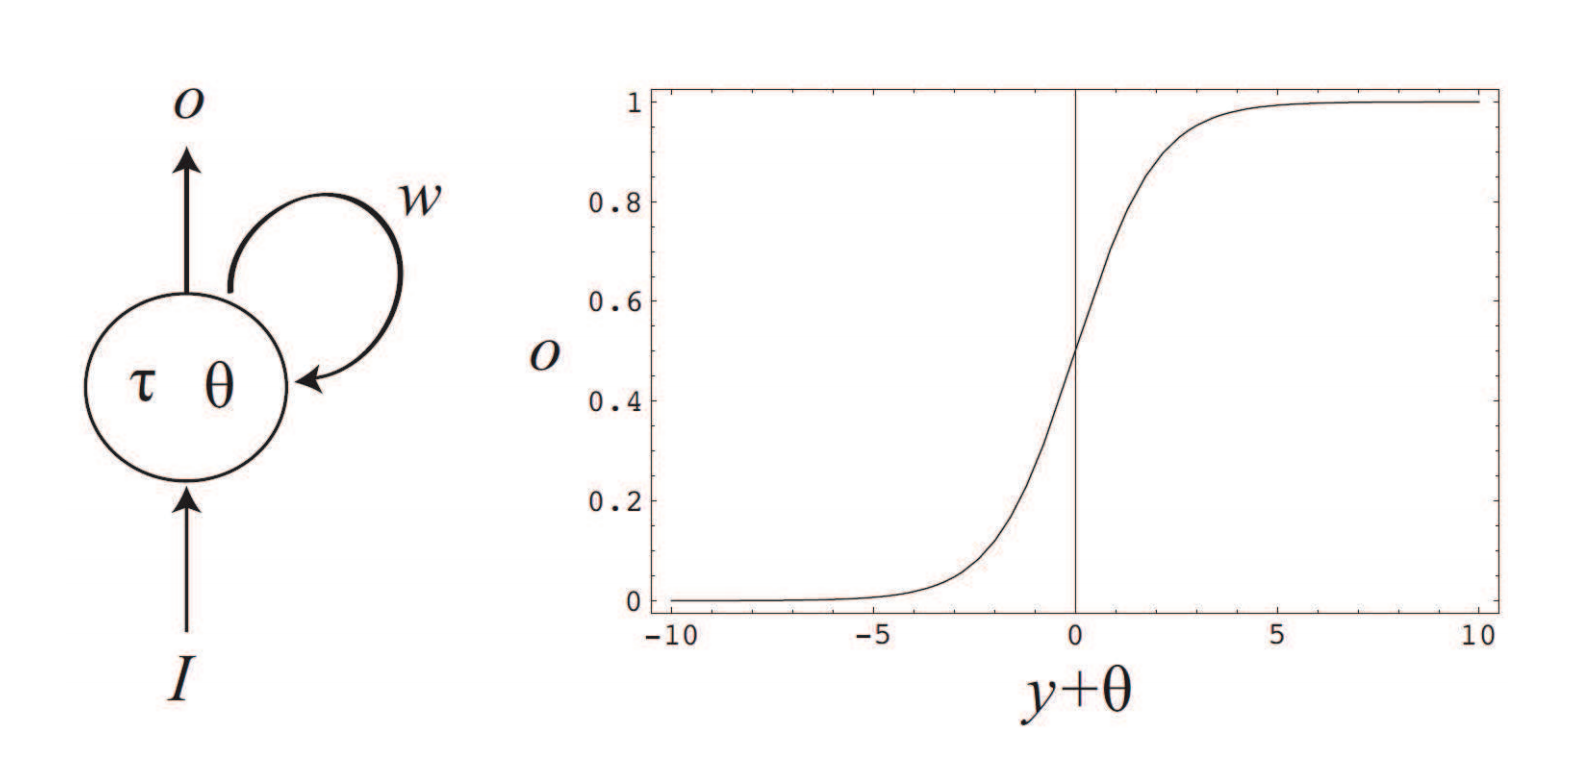
\includegraphics[width=0.8\textwidth,height=6cm]{Imagenes/CTRNNBasica}
    \caption{Valor de salida de una CTRNN. \textbf{Izquierda:} Un nodo autoconectado. \textbf{Derecha:} Función sigmoide aplicada para calcular la salida de una neurona.}
    \label{fig:figuraCTRNNBasica}
\end{figure}

En cuanto al valor de activación, a diferencia de una red neuronal feed-forward, la cual realiza
un mapeo directo entre entrada y salida de la red, el comportamiento de una CTRNN corresponde
al de un sistema dinámico (Beer, 1995a), por lo que el valor de activación de la neurona convergerá
a un punto de equilibrio. Para el análisis de las dinámicas del sistema formado por el agente
controlado por la CTRNN y el entorno, se analizarán sus diagramas de bifurcación, los cuales
muestran todos los puntos de equilibrio para la activación de las neuronas de la red.

\section{Homeostasis, ultraestabilidad y plasticidad}
La ultraestabilidad del agente se ha conseguido dotando al mismo de mecanismos de plasticidad, que le permiten modificar los valores de algunos de sus atributos internos. En este caso, los agentes pueden
alterar los valores de los pesos $w_{ij}$ de las conexiones entre las neuronas de la red cuando la frecuencia de activación de una neurona es demasiado baja o demasiado alta.

La homeostasis no se encuentra programada explícitamente, pero aparece de forma implícita debido a los mecanismos de evaluación de la evolución genética que recompensan con mejor puntuación a aquellos
agentes que, durante la realización del entrenamiento, han mantenido un mayor número de sus neuronas estables.

La plasticidad de cada conexión esta gobernada por la actividad sináptica de la conexión junto con una regla de plasticidad codificada genéticamente. Estas reglas de plasticidad vienen dadas por las
ecuaciones 3.3, 3.4, 3.5 y 3.6, donde $\Delta w_{ij}$ es el incremento por unidad de tiempo de un determinado peso sináptico ($w_{ij}$), y $z_{i}$ y $z_{j}$ son las frecuencias de
activación de las neuronas presinápticas y postsinápticas respectivamente.

Las reglas de plasticidad se construyen en torno a cuatro parámetros: la frecuencia de aprendizaje ($n_{ij}$), un valor límite ($z_{ij}^{o}$), el grado de facilitación plástica local ($p_{j}$) y
un factor de amortiguación linear que restringe el cambio dentro de los limites establecidos para los valores de los pesos sinápticos ($\delta$).

\noindent
R0: Sin plasticidad:
\begin{equation} \label{eq:R0plasticityRule}
 \centering
 \Delta w_{ij}= 0
\end{equation}
\noindent
R1: Aprendizaje Hebbiano acotado:
\begin{equation} \label{eq:R1plasticityRule}
 \centering
 \Delta w_{ij}= \delta n_{ij} p_{j} z_{i} z_{j}
\end{equation}
\noindent
R2: Potenciación o depresión amortiguadas de la neurona presináptica cuando la eficacia sináptica es muy alta o muy baja:
\begin{equation} \label{eq:R2plasticityRule}
 \centering
 \Delta w_{ij}= \delta n_{ij} p_{j} (z_{i} - z_{ij}^{o}) z_{j}
\end{equation}
\noindent
R3: Potenciación o depresión amortiguadas de la neurona postsináptica cuando la eficacia sináptica es muy alta o muy baja:
\begin{equation} \label{eq:R3plasticityRule}
 \centering
 \Delta w_{ij}= \delta n_{ij} p_{j} z_{i} (z_{j} - z_{ij}^{o})
\end{equation}

El grado de facilitación plástica local ($p_{j}$) se ve incrementado linealmente (hasta un valor máximo de 1) cuando la frecuencia de activación aumenta hasta salirse de sus límites, facilitando
así los cambios plásticos. Cuando la frecuencia de activación entra en sus límites, $p_{j}$ decrece linealmente (hasta un valor mínimo de -1), disminuyendo la facilidad de los cambios plásticos.

El cambio en la conexión sináptica depende del signo de $n_{ij}$, de forma que cada neurona puede actuar de manera independiente facilitando los cambios plásticos en la dirección indicada.

El factor de amortiguación lineal ($\delta$) asegura que los valores de los pesos se mantienen dentro de los límites establecidos para ellos.

El factor de valor límite ($z_{ij}^{o}$) depende linealmente del valor actual del peso que se está actualizando plásticamente, por lo que es calculado en cada modificación.

Los pesos son actualizados cada iteración (si precede, dependiendo de su regla de plasticidad) a partir de la ecuación 3.7.
\begin{equation} \label{eq:WeightUpdate}
 \centering
 w_{ij}(t+1) = w_{ij}(t) + \Delta w_{ij}
\end{equation}

\section{Agente}
TODO: Hablar de la forma del agente y de las configuraciones elegidas en temas de rangos y plasticidades

\subsubsection{Estructura de la red, simetría y rangos de valores utilizados}
La CTRNN utilizada para la realización de este experimento esta compuesta por ocho neuronas totalmente interconectadas entre sí, presentando la estructura que puede observarse en la figura 3.2.
Las dos primeras neuronas (0 y 1 en la figura 3.2) serán las que se encuentren conectadas a los dos sensores y por tanto las que reciben sus mediciones y las procesen. Las dos últimas neuronas
(6 y 7 en la figura 3.2) serán las que se encuentren conectadas a los dos motores, los cuales procesarán las salidas de estas neuronas para calcular las velocidades de cada uno de ellos.

\begin{figure}[!h]
	\centering
	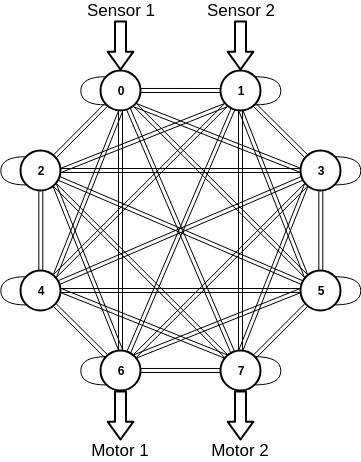
\includegraphics[width=0.4\textwidth,height=7cm]{Imagenes/MyRed}
	\caption{Esquema de la estructura de la red utilizada con 8 neuronas totalmente interconectadas.}
	\label{fig:figuraMyRed}
\end{figure}

\begin{table}[!h]
\centering
\label{table:tablaValoresParametros}
\begin{tabular}{l|l|c|c}
\textbf{Parametro} & \textbf{Descripción}          & \multicolumn{1}{l|}{\textbf{Valor mínimo}} & \multicolumn{1}{l}{\textbf{Valor máximo}} \\
\textit{$\tau_{i}$}       & Constante de decaimiento      & 0.4                                        & 4.0                                       \\
\textit{$\theta{i}$}      & Bias                          & -3.0                                       & 3.0                                       \\
\textit{Gain}      & Ganancia motora y sensora     & 0.1                                        & 10.0                                      \\
\textit{$w_{ij}$}      & Peso de la conexión sináptica & -10.0                                      & 10.0                                      \\
\textit{$n_{ij}$}     & Ritmo de plasticidad          & -0.9                                       & 0.9
\end{tabular}
\caption{Rango de valores para los parámetros de la red}
\end{table}

Para la realización de los experimentos se utilizarán CTRNNs en las que todas las neuronas
estén totalmente interconectadas (conexión de cada neurona con todas las demás en ambas direcciones) y
autoconectadas (conexión recurrente de la neurona a sí misma).

Como mínimo la CTRNN contará con cuatro neuronas. Dos de ellas conectadas cada una a uno de los dos sensores del agente y las otras dos conectadas cada una a uno de los dos motores del agente (además de
tener el resto de conexiones anteriormente descritas).

La red contará con una cierta simetría en las ganancias de las neuronas sensoras y motoras. Teniendo las dos neuronas conectadas a los sensores del agente iguales ganancias entre si, al igual que las dos neuronas conectadas
a los motores del agente.




\section{Algoritmo genético}
Hablar del algoritmo genetico utilizado, parametros, etc
Hablar de la funcion fitness utilizada

\section{Entorno de trabajo}
Python y todas las librerias utilizadas
